\documentclass[aspectratio=169,11pt]{beamer}

\usetheme{Madrid}
\usecolortheme{whale}

\setbeamertemplate{navigation symbols}{}
\setbeamertemplate{footline}{%
  \hfill\usebeamercolor[fg]{page number in head/foot}%
  \insertframenumber\,/\,\inserttotalframenumber\hspace{1em}\vspace{0.6em}}

\usepackage{booktabs}
\usepackage{xcolor}
\usepackage{pgfplots}
\pgfplotsset{compat=1.17}
\usepackage{tikz}
\usetikzlibrary{positioning,arrows.meta}
\usepackage{listings}

\definecolor{okBlue}{HTML}{0072B2}    % B0
\definecolor{okOrange}{HTML}{E69F00}  % B1
\definecolor{okGreen}{HTML}{009E73}   % B2
\definecolor{okPink}{HTML}{CC79A7}    % B3

\lstset{basicstyle=\ttfamily\footnotesize,breaklines=false,columns=fullflexible,
  keepspaces=true,frame=none,aboveskip=0.2em,belowskip=0.2em,
  literate={—}{{\textrm{---}}}1}

\newcommand{\Bz}{\textcolor{okBlue}{\textbf{B0}}}
\newcommand{\Bo}{\textcolor{okOrange}{\textbf{B1}}}
\newcommand{\Bt}{\textcolor{okGreen}{\textbf{B2}}}
\newcommand{\Bh}{\textcolor{okPink}{\textbf{B3}}}

\title{Does Verifier Feedback Help LLMs Follow Instructions?}
\subtitle{Feedback Revision on IFBench}
\author[Group {[XX]}]{Group [XX]\\[0.4em]
  {\small [Member A] ([Student ID]) \quad [Member B] ([Student ID])}\\
  {\small [Member C] ([Student ID]) \quad [Member D] ([Student ID])}}
\institute{COMP4136 Natural Language Processing\\Hong Kong Baptist University}
\date{}

\begin{document}

% 1
\begin{frame}
  \titlepage
\end{frame}

% 2
\begin{frame}{LLMs still miss verifiable output constraints}
  \begin{itemize}
    \item IFEval: 25 verifiable constraint types for instruction following [2]
    \item IFBench: 58 new out-of-domain constraints, hard for strong models [1]
    \item Self-Refine: revise outputs with the model's own feedback [3]
    \item Self-correction without external feedback is unreliable [4]
  \end{itemize}
  \vfill
  {\scriptsize
  [1] V.~Pyatkin \textit{et al.}, ``Generalizing verifiable instruction following,'' in \textit{Proc.\ NeurIPS Datasets and Benchmarks}, 2025.\par
  [2] J.~Zhou \textit{et al.}, ``Instruction-following evaluation for large language models,'' arXiv:2311.07911, 2023.\par
  [3] A.~Madaan \textit{et al.}, ``Self-Refine: Iterative refinement with self-feedback,'' in \textit{Proc.\ NeurIPS}, 2023.\par
  [4] J.~Huang \textit{et al.}, ``Large language models cannot self-correct reasoning yet,'' in \textit{Proc.\ ICLR}, 2024.\par}
\end{frame}

% 3
\begin{frame}{We test whether a verifier signal, not just a second try, fixes failures}
  \begin{itemize}
    \item RQ1: Does one revision round raise strict compliance over \Bz?
    \item RQ2: Does a verifier verdict beat self-checking (\Bt{} vs \Bo)?
    \item RQ3: Does per-constraint detail add value (\Bh{} vs \Bt)?
    \item RQ4: Which answers does revision repair, and which does it break?
  \end{itemize}
\end{frame}

% 4
\begin{frame}{Four conditions share the same prompts, models and verifier}
  \begin{columns}[T]
    \begin{column}{0.47\textwidth}
      \begin{itemize}
        \item Data: IFBench, 260 test prompts
        \item Models: gpt-4.1, gpt-4o (HKBU)
        \item Temperature 0, one revision round
        \item Metric: strict prompt-level accuracy
      \end{itemize}
    \end{column}
    \begin{column}{0.50\textwidth}
      \centering
      \begin{tabular}{ll}
        \toprule
        Condition & Revision signal \\
        \midrule
        \Bz & none (first answer) \\
        \Bo & self-check request \\
        \Bt & overall PASS / FAIL \\
        \Bh & per-constraint PASS / FAIL \\
        \bottomrule
      \end{tabular}
    \end{column}
  \end{columns}
\end{frame}

% 5
\begin{frame}{Each revision branches once from the same B0 answer}
  \centering
  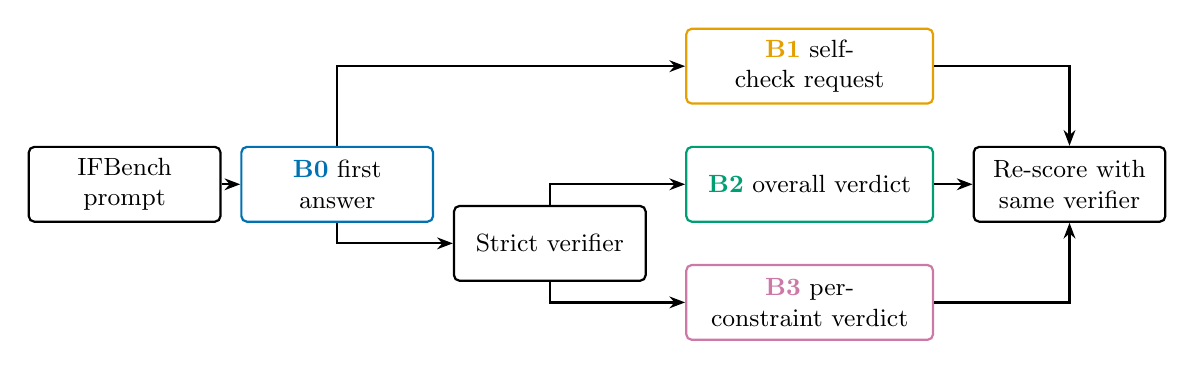
\begin{tikzpicture}[
      box/.style={draw, rounded corners=2pt, align=center, minimum height=0.95cm,
                  text width=2.2cm, font=\small, line width=0.8pt},
      wbox/.style={box, text width=2.9cm},
      arr/.style={-{Stealth[length=2mm]}, line width=0.8pt}]
    \node[box] (p) at (0,0) {IFBench prompt};
    \node[box, draw=okBlue] (b0) at (2.7,0) {\Bz{} first answer};
    \node[box] (v) at (5.4,-0.75) {Strict verifier};
    \node[wbox, draw=okOrange] (b1) at (8.7,1.5) {\Bo{} self-check request};
    \node[wbox, draw=okGreen] (b2) at (8.7,0) {\Bt{} overall verdict};
    \node[wbox, draw=okPink] (b3) at (8.7,-1.5) {\Bh{} per-constraint verdict};
    \node[box] (s) at (12.0,0) {Re-score with same verifier};
    \draw[arr] (p) -- (b0);
    \draw[arr] (b0.north) |- (b1.west);
    \draw[arr] (b0.south) |- (v.west);
    \draw[arr] (v.north) |- (b2.west);
    \draw[arr] (v.south) |- (b3.west);
    \draw[arr] (b1.east) -| (s.north);
    \draw[arr] (b2.east) -- (s.west);
    \draw[arr] (b3.east) -| (s.south);
  \end{tikzpicture}
\end{frame}

% 6
\begin{frame}{B2 reaches the highest accuracy on both models}
  \centering
  \begin{tabular}{lcccc}
    \toprule
     & \multicolumn{2}{c}{gpt-4.1} & \multicolumn{2}{c}{gpt-4o} \\
    \cmidrule(lr){2-3}\cmidrule(lr){4-5}
    Condition & Strict (\%) & Loose (\%) & Strict (\%) & Loose (\%) \\
    \midrule
    \Bz{} first answer        & 53.3 & 59.8 & 57.1 & 62.9 \\
    \Bo{} self-check          & 56.4 & 62.9 & 60.6 & 65.3 \\
    \Bt{} overall verdict     & \textbf{62.9} & \textbf{67.2} & \textbf{67.2} & \textbf{71.0} \\
    \Bh{} per-constraint      & 59.1 & 64.5 & 64.9 & 69.1 \\
    \bottomrule
  \end{tabular}
\end{frame}

% 7
\begin{frame}{Verifier feedback lifts compliance; self-check alone does not}
  \begin{columns}[c]
    \begin{column}{0.58\textwidth}
      \centering
      \begin{tikzpicture}
        \begin{axis}[
          ybar, bar width=14pt,
          ymin=0, ymax=12,
          ylabel={Paired gain over B0 (pp)},
          symbolic x coords={gpt-4.1, gpt-4o},
          xtick=data,
          axis lines*=left, tick align=outside,
          width=\textwidth, height=0.62\textheight,
          enlarge x limits=0.45,
          nodes near coords, nodes near coords style={font=\scriptsize, /pgf/number format/.cd, fixed, precision=2, fixed zerofill},
          legend style={at={(0.5,1.03)}, anchor=south, legend columns=3,
                        draw=none, font=\small},
        ]
          \addplot[fill=okOrange, draw=okOrange] coordinates {(gpt-4.1,3.09) (gpt-4o,3.47)};
          \addplot[fill=okGreen,  draw=okGreen]  coordinates {(gpt-4.1,9.65) (gpt-4o,10.04)};
          \addplot[fill=okPink,   draw=okPink]   coordinates {(gpt-4.1,5.79) (gpt-4o,7.72)};
          \legend{B1, B2, B3}
        \end{axis}
      \end{tikzpicture}
    \end{column}
    \begin{column}{0.40\textwidth}
      \begin{itemize}
        \item \Bt, \Bh: significant, both models
        \item \Bo: not significant
        \item Robust to missing-data handling
      \end{itemize}
    \end{column}
  \end{columns}
\end{frame}

% 8
\begin{frame}{B2 beats B1 mainly by not breaking answers that already pass}
  \begin{itemize}
    \item Regression on passing \Bz: \Bo{} 13.8\% / 10.8\% vs \Bt{} 5.1\% / 6.8\%
    \item \Bo{} rewrites 123 of 138 passing answers; \Bt{} keeps 103 (gpt-4.1)
    \item \Bt{} = verdict + permission to keep a passing answer
    \item \Bh{} vs \Bt: no significant difference, too few items; keep simpler \Bt
  \end{itemize}
\end{frame}

% 9
\begin{frame}[fragile]{Real cases: B1 breaks a passing answer, B2 repairs a failed one}
  \textbf{gpt-4o, item 296: no whitespace allowed}\par\smallskip
  \begin{tabular}{@{}ll@{}}
    Prompt & \lstinline!...are all sets classes? The output should not contain any whitespace.! \\
    \Bz{} PASS & \lstinline!Yes—ineverydayclass-theoreticusage,everysetisaclass;someclassesarenotsets.! \\
    \Bo{} FAIL & \lstinline!Inclass theories suchasNBG,everysetisaclass,butnot everyclassisaset.! \\
    \Bt{} PASS & \lstinline!Yes:everysetisaclass,butnotallclassesaresets.! \\
  \end{tabular}
  \vspace{1.2em}

  \textbf{gpt-4.1, item 173: stop words at most 20\%}\par\smallskip
  \begin{tabular}{@{}ll@{}}
    Prompt & \lstinline!...Ensure that stop words constitute no more than 20% of the total words...! \\
    \Bz{} FAIL & \lstinline!No. Let \(B_n(x)=x^n\). For each \(x<1\), \(B_n(x)\to0\), ...! \\
    \Bt{} PASS & \lstinline!No. Choose \(B_n(x)=x^n\). Pointwise limit: \(f(x)=0\) for \(x<1\), ...! \\
  \end{tabular}
\end{frame}

% 10
\begin{frame}{A pass/fail verdict is a simple and reliable revision signal}
  \begin{itemize}
    \item Verdict plus ``keep if passed'' gives the best compliance gain
    \item Scope: two gateway models, one round, single run at temperature 0
    \item Content review of all 2080 answers near ceiling; single-rater; deviations in report
  \end{itemize}
  \vspace{1.2em}
  \textbf{Contributions:} [Member A] code; [Member B] runs; [Member C] analysis; [Member D] report
\end{frame}

\end{document}
